\documentclass[tikz]{standalone}
\usepackage{pgfplots}
\pgfplotsset{compat=1.15}
\usepackage{mathrsfs}
\usetikzlibrary{arrows,calc}
\usepackage{tkz-euclide}

\usepackage{fp}
\pagestyle{empty}

\definecolor{AngleClr}{rgb}{0,0.39215686274509803,0}
\definecolor{ShapeClr}{rgb}{0.6,0.2,0}

\begin{document}

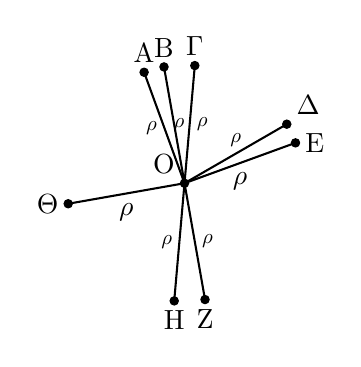
\begin{tikzpicture}[scale=.75]
\tkzSetUpLine[line width=1pt,color=black]
\tkzSetUpPoint[fill=black]

\tkzDefPoints{0/0/O,2/0/X}

\tkzDefPoint(110:2){A}
\tkzDefPoint(100:2){B}
\tkzDefPoint(85:2){C}
\tkzDefPoint(30:2){D}
\tkzDefPoint(20:2){E}
\tkzDefPoint(-80:2){F}
\tkzDefPoint(-95:2){G}
\tkzDefPoint(-170:2){H}


\tkzDrawSegments[line width=0.75pt,color=black](O,A O,B O,C O,D O,E O,F O,G O,H)

\tkzLabelSegments(O,E O,H){$\rho$}
\tkzLabelSegments[scale=0.75,above](O,D){$\rho$}
\tkzLabelSegments[scale=0.75,right](O,C O,F){$\rho$}
\tkzLabelSegments[scale=0.75,right=-0.1cm](O,B){$\rho$}
\tkzLabelSegments[scale=0.75,left](O,A O,G){$\rho$}


\tkzDrawPoints[size=3](A,B,C,D,E,F,G,H,O)
\tkzLabelPoint[above](A){$\rm A$}
\tkzLabelPoint[above](B){$\rm B$}
\tkzLabelPoint[above](C){$\rm \Gamma$}

\tkzLabelPoint[above right](D){$\rm \Delta$}
\tkzLabelPoint[right](E){$\rm E$}

\tkzLabelPoint[below](F){$\rm Z$}
\tkzLabelPoint[below](G){$\rm H$}
\tkzLabelPoint[left](H){$\rm \Theta$}

\tkzLabelPoint[above left](O){$\rm O$}


\end{tikzpicture}

\end{document}
